\section{Proceso de comisi�n disciplinaria en la Facultad 4}\label{process}
%TODO
%Descripci�n del proceso de comisi�n disciplinaria en la Facultad 4
El proceso de comisi�n disciplinaria estudiantil comienza cuando un profesor o estudiante de la \uci presenta una denuncia ante el Decano de la Facultad. La Direcci�n de la Facultad es la encargada de verificar la veracidad de la denuncia y de asignar una comisi�n disciplinaria para que investigue el caso. La comisi�n disciplinaria es la encargada de realizar la investigaci�n y de emitir conclusiones para cada infractor. Dichas conclusiones son revisadas por el Decano de la Facultad, el cual, de aceptar las conclusiones, emite la resoluci�n del caso y notifica a cada infractor.
\begin{figure}[h]
	\centering
	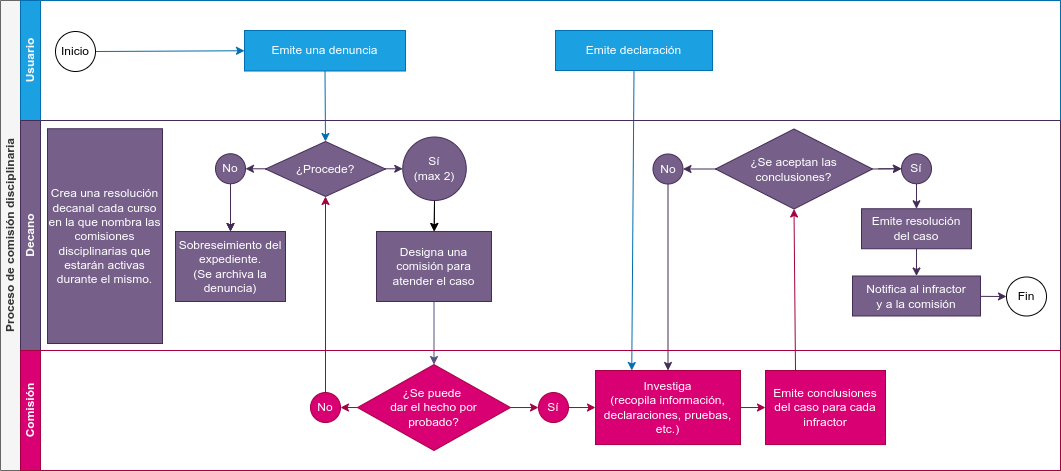
\includegraphics[width=1\textwidth]{images/process.png}
	\caption{Diagrama de carriles de piscina que modela el \proceso}
	\label{fig:entities}
\end{figure}

